% Template for PLoS
% Version 3.5 March 2018
%
% % % % % % % % % % % % % % % % % % % % % %
%
% -- IMPORTANT NOTE
%
% This template contains comments intended 
% to minimize problems and delays during our production 
% process. Please follow the template instructions
% whenever possible.
%
% % % % % % % % % % % % % % % % % % % % % % % 
%
% Once your paper is accepted for publication, 
% PLEASE REMOVE ALL TRACKED CHANGES in this file 
% and leave only the final text of your manuscript. 
% PLOS recommends the use of latexdiff to track changes during review, as this will help to maintain a clean tex file.
% Visit https://www.ctan.org/pkg/latexdiff?lang=en for info or contact us at latex@plos.org.
%
%
% There are no restrictions on package use within the LaTeX files except that 
% no packages listed in the template may be deleted.
%
% Please do not include colors or graphics in the text.
%
% The manuscript LaTeX source should be contained within a single file (do not use \input, \externaldocument, or similar commands).
%
% % % % % % % % % % % % % % % % % % % % % % %
%
% -- FIGURES AND TABLES
%
% Please include tables/figure captions directly after the paragraph where they are first \cited in the text.
%
% DO NOT INCLUDE GRAPHICS IN YOUR MANUSCRIPT
% - Figures should be uploaded separately from your manuscript file. 
% - Figures generated using LaTeX should be extracted and removed from the PDF before submission. 
% - Figures containing multiple panels/subfigures must be combined into one image file before submission.
% For figure citations, please use "Fig" instead of "Figure".
% See http://journals.plos.org/plosone/s/figures for PLOS figure guidelines.
%
% Tables should be cell-based and may not contain:
% - spacing/line breaks within cells to alter layout or alignment
% - do not nest tabular environments (no tabular environments within tabular environments)
% - no graphics or colored text (cell background color/shading OK)
% See http://journals.plos.org/plosone/s/tables for table guidelines.
%
% For tables that exceed the width of the text column, use the adjustwidth environment as illustrated in the example table in text below.
%
% % % % % % % % % % % % % % % % % % % % % % % %
%
% -- EQUATIONS, MATH SYMBOLS, SUBSCRIPTS, AND SUPERSCRIPTS
%
% IMPORTANT
% Below are a few tips to help format your equations and other special characters according to our specifications. For more tips to help reduce the possibility of formatting errors during conversion, please see our LaTeX guidelines at http://journals.plos.org/plosone/s/latex
%
% For inline equations, please be sure to include all portions of an equation in the math environment.  For example, x$^2$ is incorrect; this should be formatted as $x^2$ (or $\mathrm{x}^2$ if the romanized font is desired).
%
% Do not include text that is not math in the math environment. For example, CO2 should be written as CO\textsubscript{2} instead of CO$_2$.
%
% Please add line breaks to long display equations when possible in order to fit size of the column. 
%
% For inline equations, please do not include punctuation (commas, etc) within the math environment unless this is part of the equation.
%
% When adding superscript or subscripts outside of brackets/braces, please group using {}.  For example, change "[U(D,E,\gamma)]^2" to "{[U(D,E,\gamma)]}^2". 
%
% Do not use \cal for caligraphic font.  Instead, use \mathcal{}
%
% % % % % % % % % % % % % % % % % % % % % % % % 
%
% Please contact latex@plos.org with any questions.
%
% % % % % % % % % % % % % % % % % % % % % % % %

\documentclass[10pt,letterpaper]{article}
\usepackage[top=0.85in,left=2.75in,footskip=0.75in]{geometry}

% amsmath and amssymb packages, useful for mathematical formulas and symbols
\usepackage{amsmath,amssymb}

% Use adjustwidth environment to exceed column width (see example table in text)
\usepackage{changepage}

% Use Unicode characters when possible
\usepackage[utf8x]{inputenc}

% textcomp package and marvosym package for additional characters
\usepackage{textcomp,marvosym}

% \cite package, to clean up citations in the main text. Do not remove.
\usepackage{cite}

% Use nameref to \cite supporting information files (see Supporting Information section for more info)
\usepackage{nameref,hyperref}

% line numbers
\usepackage[right]{lineno}

% ligatures disabled
\usepackage{microtype}
\DisableLigatures[f]{encoding = *, family = * }

% color can be used to apply background shading to table cells only
\usepackage[table]{xcolor}

% array package and thick rules for tables
\usepackage{array}

% create "+" rule type for thick vertical lines
\newcolumntype{+}{!{\vrule width 2pt}}

% create \thickcline for thick horizontal lines of variable length
\newlength\savedwidth
\newcommand\thickcline[1]{%
  \noalign{\global\savedwidth\arrayrulewidth\global\arrayrulewidth 2pt}%
  \cline{#1}%
  \noalign{\vskip\arrayrulewidth}%
  \noalign{\global\arrayrulewidth\savedwidth}%
}

% \thickhline command for thick horizontal lines that span the table
\newcommand\thickhline{\noalign{\global\savedwidth\arrayrulewidth\global\arrayrulewidth 2pt}%
\hline
\noalign{\global\arrayrulewidth\savedwidth}}


% Remove comment for double spacing
%\usepackage{setspace} 
%\doublespacing

% Text layout
\raggedright
\setlength{\parindent}{0.5cm}
\textwidth 5.25in 
\textheight 8.75in

% Bold the 'Figure #' in the caption and separate it from the title/caption with a period
% Captions will be left justified
\usepackage[aboveskip=1pt,labelfont=bf,labelsep=period,justification=raggedright,singlelinecheck=off]{caption}
\renewcommand{\figurename}{Fig}


% Remove brackets from numbering in List of References
\makeatletter
\renewcommand{\@biblabel}[1]{\quad#1.}
\makeatother



% Header and Footer with logo
\usepackage{lastpage,fancyhdr,graphicx}
\usepackage{epstopdf}
%\pagestyle{myheadings}
\pagestyle{fancy}
\fancyhf{}
%\setlength{\headheight}{27.023pt}
%\lhead{\includegraphics[width=2.0in]{PLOS-submission.eps}}
\rfoot{\thepage/\pageref{LastPage}}
\renewcommand{\headrulewidth}{0pt}
\renewcommand{\footrule}{\hrule height 2pt \vspace{2mm}}
\fancyheadoffset[L]{2.25in}
\fancyfootoffset[L]{2.25in}
\lfoot{\today}

%% Include all macros below

\newcommand{\lorem}{{\bf LOREM}}
\newcommand{\ipsum}{{\bf IPSUM}}

%% END MACROS SECTION


\begin{document}
\vspace*{0.2in}

% Title must be 250 characters or less.
\begin{flushleft}
{\Large
\textbf\newline{Models and modelling practices for assessing the impact of outbreak response interventions to human vaccine-preventable diseases (1970-2019): A systematic review}
}
\newline
\\
James M. Azam\textsuperscript{1*},
Xiaoxi Pang\textsuperscript{2},
Elisha B. Are\textsuperscript{1, 3},
Juliet R.C. Pulliam\textsuperscript{1},
Matthew J. Ferrari\textsuperscript{4}
\\
\bigskip
\textbf{1} DSI-NRF Centre of Excellence in Epidemiological Modelling and Analysis (SACEMA), Stellenbosch University, Stellenbosch 7600, South Africa
\\
\textbf{2} Department of Mathematics, The University of Manchester, Manchester, UK
\\
\textbf{3} Department of Mathematics, Simon Fraser University, Burnaby, BC, Canada
\\
\textbf{4} Center for Infectious Disease Dynamics, Department of Biology, The Pennsylvania
State University, University Park, Pennsylvania, USA
\\
\bigskip

* jamesazam@sun.ac.za

\end{flushleft}
\section*{Abstract}
\subsection*{Background}
Mathematical modelling can aid outbreak response decision-making. However, this would require collaboration among model developers, decision-makers, and local experts to incorporate appropriate realism. We conducted a systematic review of modelling studies on human vaccine-preventable disease (VPD) outbreaks to identify patterns in modelling practices among collaborations. We complemented this with a mini review of eligible studies from the foot-and-mouth disease (FMD) literature.   
\subsection*{Methods}
Three databases were searched for studies published during 1970-2019 that applied models to assess the impact of an outbreak response. Per included study, we extracted data on author affiliation type (academic institution, governmental, and non-governmental organizations), whether at least one author was affiliated to the country studied, interventions, and model characteristics. Furthermore, the studies were grouped into two collaboration types: purely academic (papers with only academic affiliations), and mixed (all other combinations) to help investigate differences in modelling patterns between collaboration types in the human disease literature. Additionally, we compared modelling practices between the human VPD and FMD literature. 
\subsection*{Results}
Human VPDs formed 228 of 253 included studies. Purely academic collaborations dominated the human disease studies (56\%). Notably, mixed collaborations increased in the last seven years (2013 - 2019). Most studies had an author in the country studied (75.2\%) but this was more likely among the mixed collaborations. Contrasted to the human VPDs, mixed collaborations dominated the FMD literature (56\%). Furthermore, FMD studies more often had an author affiliated to the country studied (92\%) and used complex model design, including stochasticity, and model parametrization and validation. 
\subsection*{Conclusion}
The increase in mixed collaboration studies over the past seven years could suggest an increase in the uptake of modelling for outbreak response decision-making. We encourage more mixed collaborations between academic and non-academic institutions and the involvement of locally affiliated authors to help ensure that the studies suit local contexts.

\subsection*{Keywords}
Infectious disease dynamics; outbreak response modelling

\section*{Highlights}
\begin{enumerate}
	\item We explored the nature of collaborative modelling in the human-vaccine preventable disease outbreak response literature.
	\item Author collaborations were grouped into purely academic and mixed types.
	\item Purely academic collaborations dominated the human vaccine-preventable diseases literature.
	\item Mixed collaborations were more likely to involve local experts and use complex methods.
	\item Mixed collaborations have more potential to lead to decision-making and are recommended.
\end{enumerate}


%\subsection*{Registration}
%A protocol following the PRISMA guidelines for systematic review protocols and outlining the procedures for this systematic review was registered on PROSPERO with registration number CRD42020160803 and published through a peer-reviewed process. 
\linenumbers

\section*{Introduction}
Successful outbreak response to infectious diseases is often the result of a highly collaborative process~\cite{Sigfrid2020}. Decision-making during outbreak response usually requires collaborations between academic and field experts, including governmental and Non-Governmental Organizations (NGOs)~\cite{Kretzschmar2020,Kerkhove2012,Okiror2021,Whitty2014,Sigfrid2020}. These collaborations ensure that important perspectives from both research and operations/implementation are accounted for in the decision-making process. 

Outbreak response decision-making often requires adaptations to the affected location ~\cite{Whitty2014,Heesterbeek2015,Sigfrid2020}. The interventions and decisions are usually driven by data/evidence, information, and experiences from the past or in real-time, either locally or from similar phenomena elsewhere ~\cite{Abramowitz2015,Kerkhove2012}. Furthermore, involving local experts in the design of interventions has been found to boost the success of outbreak response efforts ~\cite{Sigfrid2020}. Consequently, outbreak response teams should ideally involve at least one local expert to provide more context~\cite{Sigfrid2020}.  

Mathematical modelling can support outbreak response decision-making~\cite{Lofgren2015}. Modelling is a proven tool for revealing insights about the extent of disease spread, and impact of interventions, while drawing on lessons learnt to provide recommendations for decision-making during outbreaks~\cite{Kretzschmar2020,Whitty2014,Lofgren2015}. Insights from mathematical modelling, though often useful, only form part of the larger context (socio-economic, political, and so forth) to be considered during an outbreak, making it difficult to determine the extent to which it contributes to outbreak response decision-making ~\cite{Kretzschmar2020,Kerkhove2012}. One way to help ensure that modelling contributes to decision-making could be through the conduct of interdisciplinary research between model developers and decision-makers.

The link between interdisciplinarity in scientific research --- that is, research conducted by authors with diverse scientific backgrounds --- and research impact, for example, number of citations has been well-researched~\cite{Abramo2017,Wagner2011}. However, few studies have investigated the impact of interdisciplinary collaborations on the conduct of scientific research. One such study investigated the impact of interdisciplinarity on the scientific validity of the methods used in a selection of papers that applied machine learning on topics in biology or medicine~\cite{Littmann2020}. The study found that the methods used in the reviewed studies differed according to the nature of the scientific backgrounds of the authors who conducted the research. Our preliminary searches of the literature did not reveal any of such review studies investigating differences in research practices among collaborations in the outbreak response modelling literature. We, therefore, conducted a systematic review of outbreak response modelling studies of human vaccine-preventable diseases with the goal to explore the time and geographic (countries) patterns of collaboration types, and to ascertain differences in practices between the collaboration types in terms of the choice of model characteristics, modelling methods, and other topics. 

We sought to answer the following questions with respect to the collaboration landscape in the human disease outbreak response modelling literature: (1) How are the studies distributed in time and geographic locations, and how often is at least one of the collaborators geographically connected to the location being studied? (2) What types of interventions are generally modelled and is there a difference between the conclusions drawn about the impact of interventions, especially, vaccination in comparison with other non-vaccination interventions during outbreaks? (3) Do the model characteristics (structure and dynamics) and modelling practices (parametrization, validation, and so forth) differ between the collaboration types?    

We acknowledge that there is a parallel body of relevant modelling work in the livestock literature. Specifically, the outbreak response effort that resulted from the 2001 foot-and-mouth disease (FMD) virus outbreak in the United Kingdom has been a foundational example of the application of mathematical modelling for decision-making. Subsequent work based on this outbreak has been instrumental in the development of FMD outbreak intervention strategies around the world. Hence, even though the primary scope of this review is the application of models to inform outbreak response for human infectious diseases, we include the relevant FMD references for comparison. In the end, we, therefore, study the differences in terms of collaborations in the human disease modelling literature, and compare our observations to that of the FMD modelling literature to further ascertain any differences in approaches and practices between the human and livestock literature. 


%The following were the objectives of the systematic review:
%\begin{enumerate}
%	\item To ascertain differences in model characteristics and modelling methods between collaboration types. 
%	\item To determine the distribution of outbreak response modelling studies over time (years) overall and in terms of collaboration types, 
%	\item To determine how often at least one of the authors on a paper was geographically connected to the country/location studied and whether there were differences between collaboration types,
%	\item To investigate types of interventions modelled and differences between the conclusions drawn about the impact of interventions.
%\end{enumerate}
   

\section*{Materials and methods}
We followed the 2020 Preferred Reporting Items for Systematic Reviews and Meta-analyses statement (PRISMA 2020)  to conduct this systematic review \cite{Page2021}.

\subsection*{Eligibility criteria}
The following definitions were used in the determining study eligibility:

\begin{itemize}
	\item ``Outbreak'': a new and sudden rise in the number of cases of a disease in a population, which when left uncontrolled, could lead to large scale geographic spread, AND 
	\item ``Outbreak response'': an intervention directly triggered by the outbreak of an infectious disease, AND
	\item ``Mechanistic models'': mathematical models that use an equation or system of equations to capture the biological mechanisms driving the transmission dynamics of the infectious disease at the level of an individual or population \cite{Lessler2016a,Reiner2013}, AND
	\item ``Outbreak intervention assessment'': a mechanistic model-based evaluation of the impact of an outbreak response intervention.
\end{itemize}

We included studies that used a mechanistic model to investigate the impact of interventions triggered by the outbreak of any of the human vaccine-preventable diseases we considered (Table 1 in \nameref{S1_File}), Ebola, or foot-and-mouth disease. Studies were considered unique even if they had a duplicated author list or a slight variation in the author list, probably representing the same modelling group, so far as the content of the paper was different. 


We excluded studies that satisfied at least one of the following criteria: 

\begin{itemize}
	\item Study used a model that is not mechanistic,
	\item Study is not about an outbreak as defined,
	\item Disease studied is not a human vaccine-preventable disease (Table 1 in \nameref{S1_File}), Ebola or foot-and-mouth disease,
	\item Study's objective is not to evaluate the impact of an intervention mounted in response to an outbreak, or
	\item Study is not published in English.
\end{itemize}

\subsection*{Information sources}
On January 15, 2020, we searched Scopus, PubMed, and Web of Science for eligible records. We searched each database from its earliest date of coverage through January 15, 2020. 

\subsection*{Search strategy}
We constructed and validated search strings specific to each database. To validate the search strings, we first ran them in the specific database's search engine and obtained a database of records. We then searched the database for well-known papers that fit the criteria for included studies. We did this for each disease on our list. 

The search strings were constructed by all five reviewers (JMA, XP, EBA, MJF, and JRCP) and in consultation with the Faculty of Science Librarian of Stellenbosch University to reflect three main topics and their synonyms, that is, ``outbreak'', ``intervention'', and ``mechanistic model''. 

The following are the search strings per database. 

\textbf{Scopus (Title, abstract, keywords search)}:

( TITLE-ABS-KEY ( epidemic  OR  outbreak  OR  emergency  OR  reactive  OR  crisis ) )  AND  ( TITLE-ABS-KEY ( respon*  OR  manage*  OR  control  OR  interven*  OR  strateg* ) )  AND  ( TITLE-ABS-KEY ( stochastic  OR  transmission  OR  computational  OR  mathematical  OR  mechanistic  OR  statistical  OR  simulation  OR  "In silico"  OR  dynamic* ) )  AND  ( TITLE-ABS-KEY ( model* ) )  AND  ( ( TITLE-ABS-KEY ( cholera  OR  dengue  OR  diphtheria  OR  ebola  OR  "Foot-and-mouth"  OR  "foot and mouth"  OR  fmd  OR  "Hepatitis A"  OR  "Hepatitis B"  OR  "Hepatitis E"  OR  "Haemophilus influenzae type b"  OR  hib  OR  "Human papillomavirus"  OR  hpv  OR  influenza ) )  OR  ( TITLE-ABS-KEY ( "Japanese encephalitis"  OR  malaria  OR  measles  OR  "Meningococcal meningitis"  OR  mumps  OR  pertussis  OR  "Whooping cough"  OR  "Pneumococcal disease"  OR  poliomyelitis  OR  polio  OR  rabies  OR  rotavirus  OR  rubella ) )  OR  ( TITLE-ABS-KEY ( tetanus  OR  "Tick-borne encephalitis"  OR  tuberculosis  OR  typhoid  OR  varicella  OR  chickenpox  OR  "Yellow Fever"  OR  "vaccine-preventable" ) ) )

\textbf{PubMed (Title and abstract search)}:

Search ((((((Epidemic OR Outbreak OR Emergency OR Reactive OR Crisis))) AND ((Response OR Management OR Control OR Intervention OR Strategies))) AND ((Stochastic OR Transmission OR Computational OR Mathematical OR Mechanistic OR Statistical OR Simulation OR "In silico" OR Dynamic*))) AND model*) AND ((Cholera OR Dengue OR Diphtheria OR Ebola OR "Foot-and-mouth" OR "foot and mouth" OR FMD OR "Hepatitis A" OR "Hepatitis B" OR "Hepatitis E" OR "Haemophilus influenzae type b" OR Hib OR "Human papillomavirus" OR HPV OR Influenza OR "Japanese encephalitis" OR Malaria OR Measles OR "Meningococcal meningitis" OR Mumps OR Pertussis OR "Whooping cough" OR "Pneumococcal disease" OR Poliomyelitis OR Polio OR Rabies OR Rotavirus OR Rubella OR Tetanus OR "Tick-borne encephalitis" OR Tuberculosis OR Typhoid OR Varicella OR Chickenpox OR "Yellow Fever" OR "vaccine-preventable"))

\textbf{Web of Science (Topic search)}:

TOPIC: (Epidemic OR Outbreak OR Emergency OR Reactive OR Crisis) AND TOPIC: (Respon* OR  Manage*  OR  Control  OR  Interven*  OR  Strateg*)) AND TOPIC: (Stochastic OR Transmission OR Computational OR Mathematical OR Mechanistic OR Statistical OR Simulation OR In silico OR Dynamic*) AND TOPIC: (model*) AND TOPIC: (Cholera OR Dengue OR Diphtheria OR Ebola OR "Foot-and-mouth" OR "foot and mouth" OR FMD OR "Hepatitis A" OR "Hepatitis B" OR "Hepatitis E" OR "Haemophilus influenzae type b" OR Hib OR "Human papillomavirus" OR HPV OR Influenza OR "Japanese encephalitis" OR Malaria OR Measles OR "Meningococcal meningitis" OR Mumps OR Pertussis OR "Whooping cough" OR "Pneumococcal disease" OR Poliomyelitis OR Polio OR Rabies OR Rotavirus OR Rubella OR Tetanus OR "Tick-borne encephalitis" OR Tuberculosis OR Typhoid OR Varicella OR Chickenpox OR "Yellow Fever" OR "vaccine-preventable")


\subsection*{Study selection}
We used Endnote version X7.8 and Rayyan web application (\url{https://www.rayyan.ai/}) to combine the results from the three databases and to identify and remove duplicate records. The unique records were exported into Rayyan web application, where they were screened in two stages by three reviewers (JMA, XP, and EBA). 

Stage one screening involved excluding studies based on their title and abstract, using the questionnaire that follows. The reviewers only used the information provided in the title and abstract of each study to decide whether it was eligible for inclusion (``Include''), not eligible (``Exclude''), or likely to be included (``Maybe''). The ``Include'' and ``Maybe'' category of studies further went through stage two screening described ahead, which was more stringent. 

\subsubsection*{Questionnaire for title and abstract screening (Stage 1)}
\begin{enumerate}
	\item	Is this article written in English?
	\begin{itemize}
		\item 	No: Exclude. Reason: Not English
	\end{itemize}
	\item 	Does the title of this article fit the scope of this review?
	\begin{itemize}
		\item 	No: Exclude. Reason: Title out of scope
	\end{itemize}
	\item	Does the topic of the abstract fit the scope of this review?
	\begin{itemize}
		\item 	No: Exclude. Reason: Topic out of scope
	\end{itemize}
	\item Is this study entirely a review (literature review, systematic review, scoping review, not indicated)? 
	\begin{itemize}
		\item 	Yes: Exclude. Reason: Review
	\end{itemize}
	\item Is any part of this study about an outbreak that happened in the past, was ongoing at the time of the study, or a hypothetical one, including one that could happen in the future? We define an outbreak as a new and sudden rise in the number of cases of a disease in a population, which when left uncontrolled, could lead to large scale geographic spread.
	\begin{itemize}
		\item 	No: Exclude. Reason: Not an outbreak
	\end{itemize}
	\item Is any part of this study about a human infectious disease (Table 1 in \nameref{S1_File}), Ebola or foot-and-mouth disease in livestock?
	\begin{itemize}
		\item 	No: Exclude. Reason: Disease not in scope
	\end{itemize}
	\item Does this study assess the impact – epidemiological or operational - of a real or hypothetical intervention that was mounted or could potentially be mounted in response to an outbreak of the disease in question? Note that we define an assessment as an evaluation of either the absolute or relative impact of an intervention on one of several outcomes including number/proportion of population reached with the intervention (coverage), and a change in size - number of people, duration, spatial - of the outbreak.
	\begin{itemize}
		\item 	No: Exclude. Reason: Not an outbreak intervention assessment
		\item 	Maybe. Reason: Intervention details unclear
	\end{itemize}
	\item Does this study solely use static methods for evaluating the intervention? Static methods include surveys, regression methods, descriptive, and exploratory statistical methods.
	\begin{itemize}
		\item 	No: Exclude. Reason: Not a model
	\end{itemize}
	\item Does this study use any kind of equation, system of equations, or computer simulation to capture the disease’s transmission process or natural history over time?
	\begin{itemize}
		\item 	No: Exclude. Reason: Model not mechanistic
		\item 	Maybe. Reason: Likely a model
	\end{itemize}
\end{enumerate}

Stage one was first piloted with all three reviewers screening the same 50 studies using Rayyan in ``blind mode''. This was so that the reviewers could not see each other's screening decisions (inclusion/exclusion/maybe). After the pilot screening, the results were compared and any inclusion/exclusion conflicts were discussed and resolved. The pilot phase ensured that all the reviewers were using a consistent screening approach. The remaining studies were then screened in duplicate and all conflicting decisions were resolved at the end through discussions among the reviewers. 

Stage 2 involved screening the included studies from stage 1, using their full text, in duplicate and with the following questionnaire.

\subsubsection*{Questionnaire for full text screening (Stage 2)}
\begin{enumerate}
	\item Is this article written in English? (This was necessary because some articles could have English abstracts but non-English full text)
	\begin{itemize}
		\item 	If no, exclude. Reason: Not English	
	\end{itemize}
	\item Is this article a report, commentary or any kind of non-quantitative report?
	\begin{itemize}
		\item 	If yes, exclude. Reason: Article type out of scope
	\end{itemize}
	\item Is the full text readily available?
	\begin{itemize}
		\item 	If no, mark as Maybe. Reason: Full text not available	
	\end{itemize}
	\item Is this study entirely a review (literature review, systematic review, scoping review, not indicated)? 
	\begin{itemize}
		\item 	If yes, exclude. Reason: Review
	\end{itemize}
	\item Is the study or a part of it about an outbreak, real or hypothetical?
	\begin{itemize}
		\item 	If no, exclude. Reason: Not an outbreak
	\end{itemize}
	\item Is the disease a human vaccine-preventable disease (Table 1 in \nameref{S1_File}), Ebola, or foot-and-mouth disease? 
	\begin{itemize}
		\item 	If no, exclude. Reason: Not a listed disease
	\end{itemize}
	\item Does this study solely use static methods for evaluating the intervention? Static methods include surveys, regression methods, descriptive, exploratory statistical methods.
	\begin{itemize}
		\item 	If no, exclude. Reason: Static model or method
	\end{itemize}
	\item Does this study use any kind of equation, system of equations, or computer simulation to capture the disease’s transmission process in a dynamic way?
	\begin{itemize}
		\item 	If no, exclude. Reason: Model not mechanistic
		\item 	If unclear, maybe. Reason: Likely a model
	\end{itemize}
	\item Is the model about within-host dynamics?
	\begin{itemize}
		\item 	If yes, exclude. Reason: Within-host model
	\end{itemize}
	\item Does this study attempt to assess the impact – epidemiological or operational - of a real or hypothetical intervention that was mounted or could potentially be mounted in response to an outbreak of the disease in question? We define an assessment as an evaluation of either the absolute or relative impact of an intervention on one of several outcomes including number/proportion of population reached with the intervention (coverage), and a change in size - number of people, duration, spatial - of the outbreak.
	\begin{itemize}
		\item 	If no, exclude. Reason: Not an outbreak intervention assessment
		\item 	If unclear, maybe. Label: Intervention details unclear
	\end{itemize}
\end{enumerate}

\subsection*{Data extraction}
To extract the data from the studies, we used the data extraction questionnaire implemented with the KoboToolbox web application (Section 3 in \nameref{S1_File}). The questionnaire was first piloted with 10 papers among the three reviewers, who worked in duplicate. All conflicts in terms of extracted data were resolved. 

Following the pilot phase, the full list of included studies was shared among three reviewers (JMA, XP, and EBA), who extracted the relevant data independently. The extracted data was cross-checked by one reviewer (JMA). When a discrepancy was found in the extracted data, the reviewer referred to the original paper and resolved the conflict.  

We extracted data on the type of publication, author affiliation type (academic/government/non-governmental), country/setting studied, whether at least one author affiliation was situated in the country studied, disease studied, the study objectives (retrospective/prospective impact assessment, timing of the modelling practice with respect to the outbreak (retrospective/prospective/real-time), interventions studied, and whether vaccination was the most impactful intervention when compared as a single intervention (yes/no/inconclusive). A full list of the extracted data items are provided (Section 2 in \nameref{S1_File}).  

From the model in each paper, we extracted data on the representation of individuals (compartmental vs individual-based), whether spatial structure was represented (yes/no), model structure (deterministic vs stochastic), model parameterization, and validation. We also extracted a predefined list of outcomes (cases averted, final epidemic size, etc) measured with the models. If an outcome was reported that was not on the pre-defined list, we collected it separately as free text for further analysis. We also extracted data on whether the studies included sensitivity analysis or not. This was to understand how uncertainties in the model inputs were dealt with.  We collected data on whether the studies used real world data, that is, excluding simulated data, and whether the data was openly available for download. We also extracted information on whether the code used for the analysis and visualization were made openly available.


\subsection*{Data analysis and synthesis}
To understand how the papers were distributed in terms of author affiliations, we first tallied the unique combinations of author affiliation types. We then grouped the author affiliations into the following two collaboration types and performed all further analyses by stratifying the variable(s) of interest by them:

\begin{enumerate}
	\item \textit{Purely academic:} papers with only academic author affiliations (academics collaborating with other academics), 
	\item \textit{Mixed:} papers with a mixture of academic, government and NGO affiliations. This collaboration type also included papers with only government or only NGO affiliations. 
\end{enumerate}

We first explored the trend in aggregated publications during 1970-2019 by counting the number of publications in each year irrespective of collaboration type. 

To explore how the publications changed in time with respect to the collaboration types, we tallied the number of publications and relative proportion (mixed versus purely academic collaboration) of studies per year. We lumped together the publications from 1970 to 2005 due to the small numbers. 

To study how the papers were distributed in terms of geographic locations, we split the studies into those that studied actual versus hypothetical locations and used the subset of studies about actual locations to rank the topmost studied locations (country and continent) by frequency. 

We also investigated how connected the authors were to the locations studied. Here, we only considered studies on geographic scales up to actual countries and not larger. All studies about locations larger than a country were dropped from this part of the analysis. We tallied, in terms of collaboration types, the number of studies about actual locations (countries) with or without at least one author affiliation in the studied location. If a paper studied more than one location, we treated each location as a separate instance. This increased the denominators accordingly. 

To summarize the conclusions drawn about the impact of vaccination as a single intervention, we grouped the studies into three categories, that is, studies that modelled non-vaccination interventions, those that modelled vaccination in combination with other interventions, and those that modelled vaccination as a single intervention for comparison with other interventions. The question was only applicable to the last category of interventions, so we counted the number of studies that found vaccination to be the most impactful or not. Where vaccination was not found to be the most impactful, we briefly summarised the reasons and modelling assumptions. 

For the disease studied, model characteristics (structure, dynamics, and spatial heterogeneity), and modelling practices (parametrization, validation, sensitivity analysis, data and code use and availability), we counted the number of studies per collaboration type and reported the results as percentages and fractions of the total. In counting the number of papers per disease studied and outcome measured, if a study had more than one outcome measured or disease, we treated each instance as unique and counted them separately. Hence, in such cases, the denominator of the reported fraction increased from the total studies we reported in our search results. 

To summarise the model outcomes, we stratified by the collaboration type and tallied the outcomes used within each group. We reported the top six most used outcomes by both collaboration types and compared the results between the two.

All analyses were perform in R 4.0.5 ~\cite{R2021}. We have provided a database of all the screened papers and their associated extracted data in a csv file, which can be accessed at \url{https://osf.io/dmvst/?view_only=b50a8d3ec21b4a07b7977d0f56e79fc3}. Additionally, all the analysis tables are provided as a supplement (\nameref{S2_File}). 

\section*{Results}
\subsection*{Study selection}
We retrieved a total of $12, 986$ bibliographic records from Scopus, PubMed, and Web of Science (Fig \ref{PRISMA_flowchart}). Using Endnote and Rayyan, we identified and removed $7, 974$ duplicates, resulting in $5, 012$ unique records for title, abstract, and full text screening. We exported the unique records into Rayyan for the screening in two stages. Stage 1 involved a title and abstract screening in duplicate by the three reviewers and resulted $4, 211$ excluded studies. The stage 2 screening, which involved screening the full text, led to $548$ excluded studies. 

After the full text screening, $253$ studies remained for the data extraction stage of which $228$ on human vaccine-preventable diseases and $25$ studies were on FMD. The FMD studies were only used for comparisons. 

\begin{figure}[!h]
	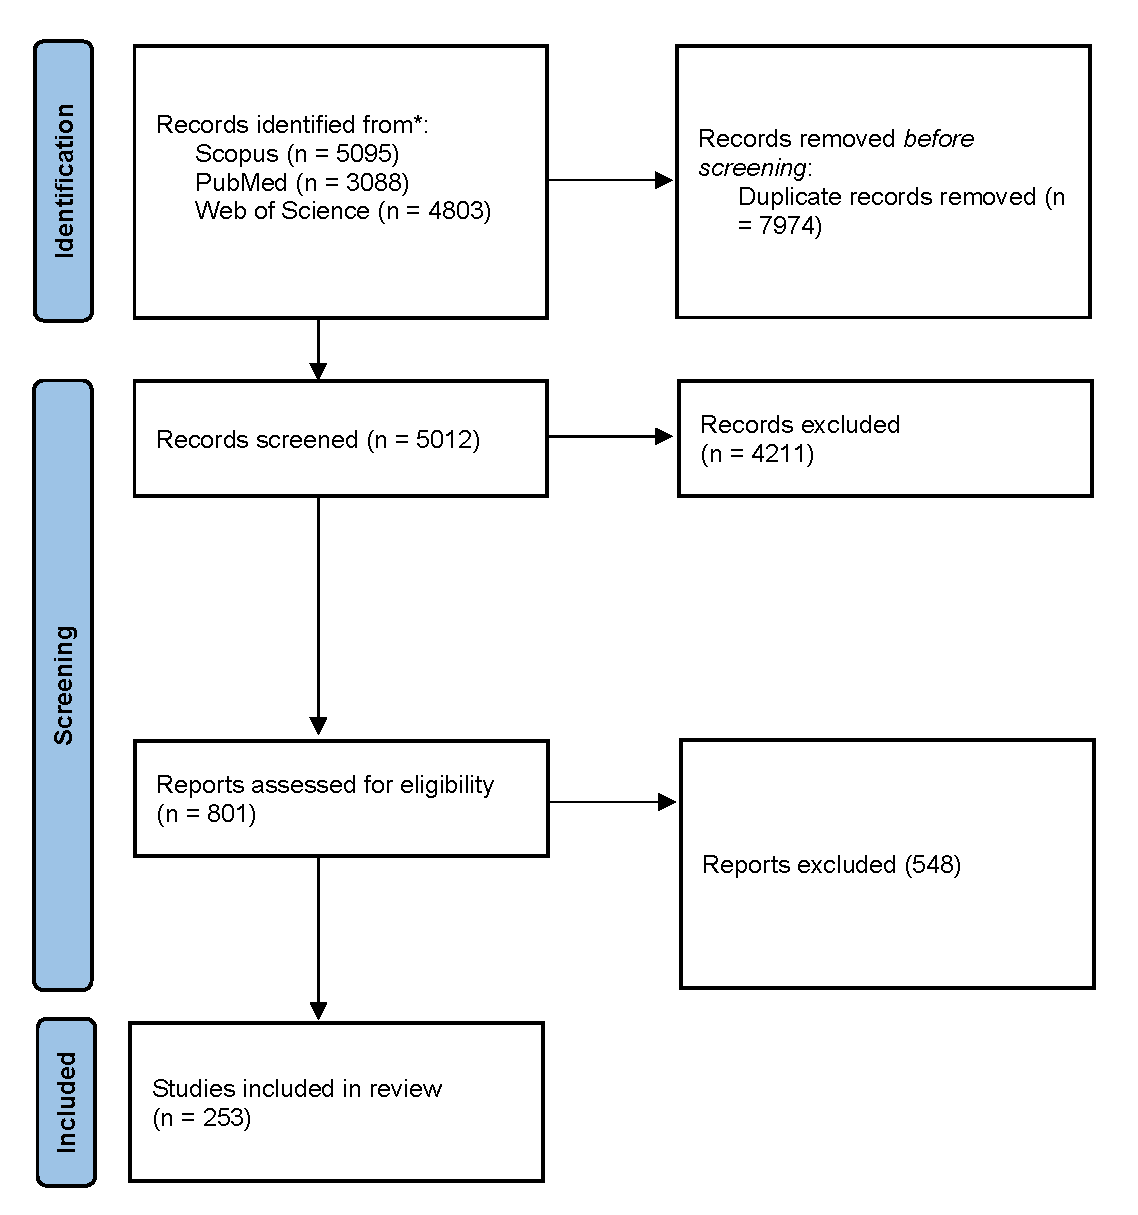
\includegraphics[scale=0.85]{figs/fig1_PRISMA_flowchart}
	\caption{\bf The PRISMA flow chart. Numbers described here include studies for both the human vaccine-preventable diseases and foot-and-mouth disease.}
	\label{PRISMA_flowchart}
\end{figure}

\subsection*{Publications over time}
Overall, a few outbreak response modelling papers were published between 1970-2005 $(3.9\%; 9/228)$, followed by a marked increase in publications until 2019 $(96.1\%; 220/228)$ (Fig \ref{publications_per_year}). 

\begin{figure}[!h]	
 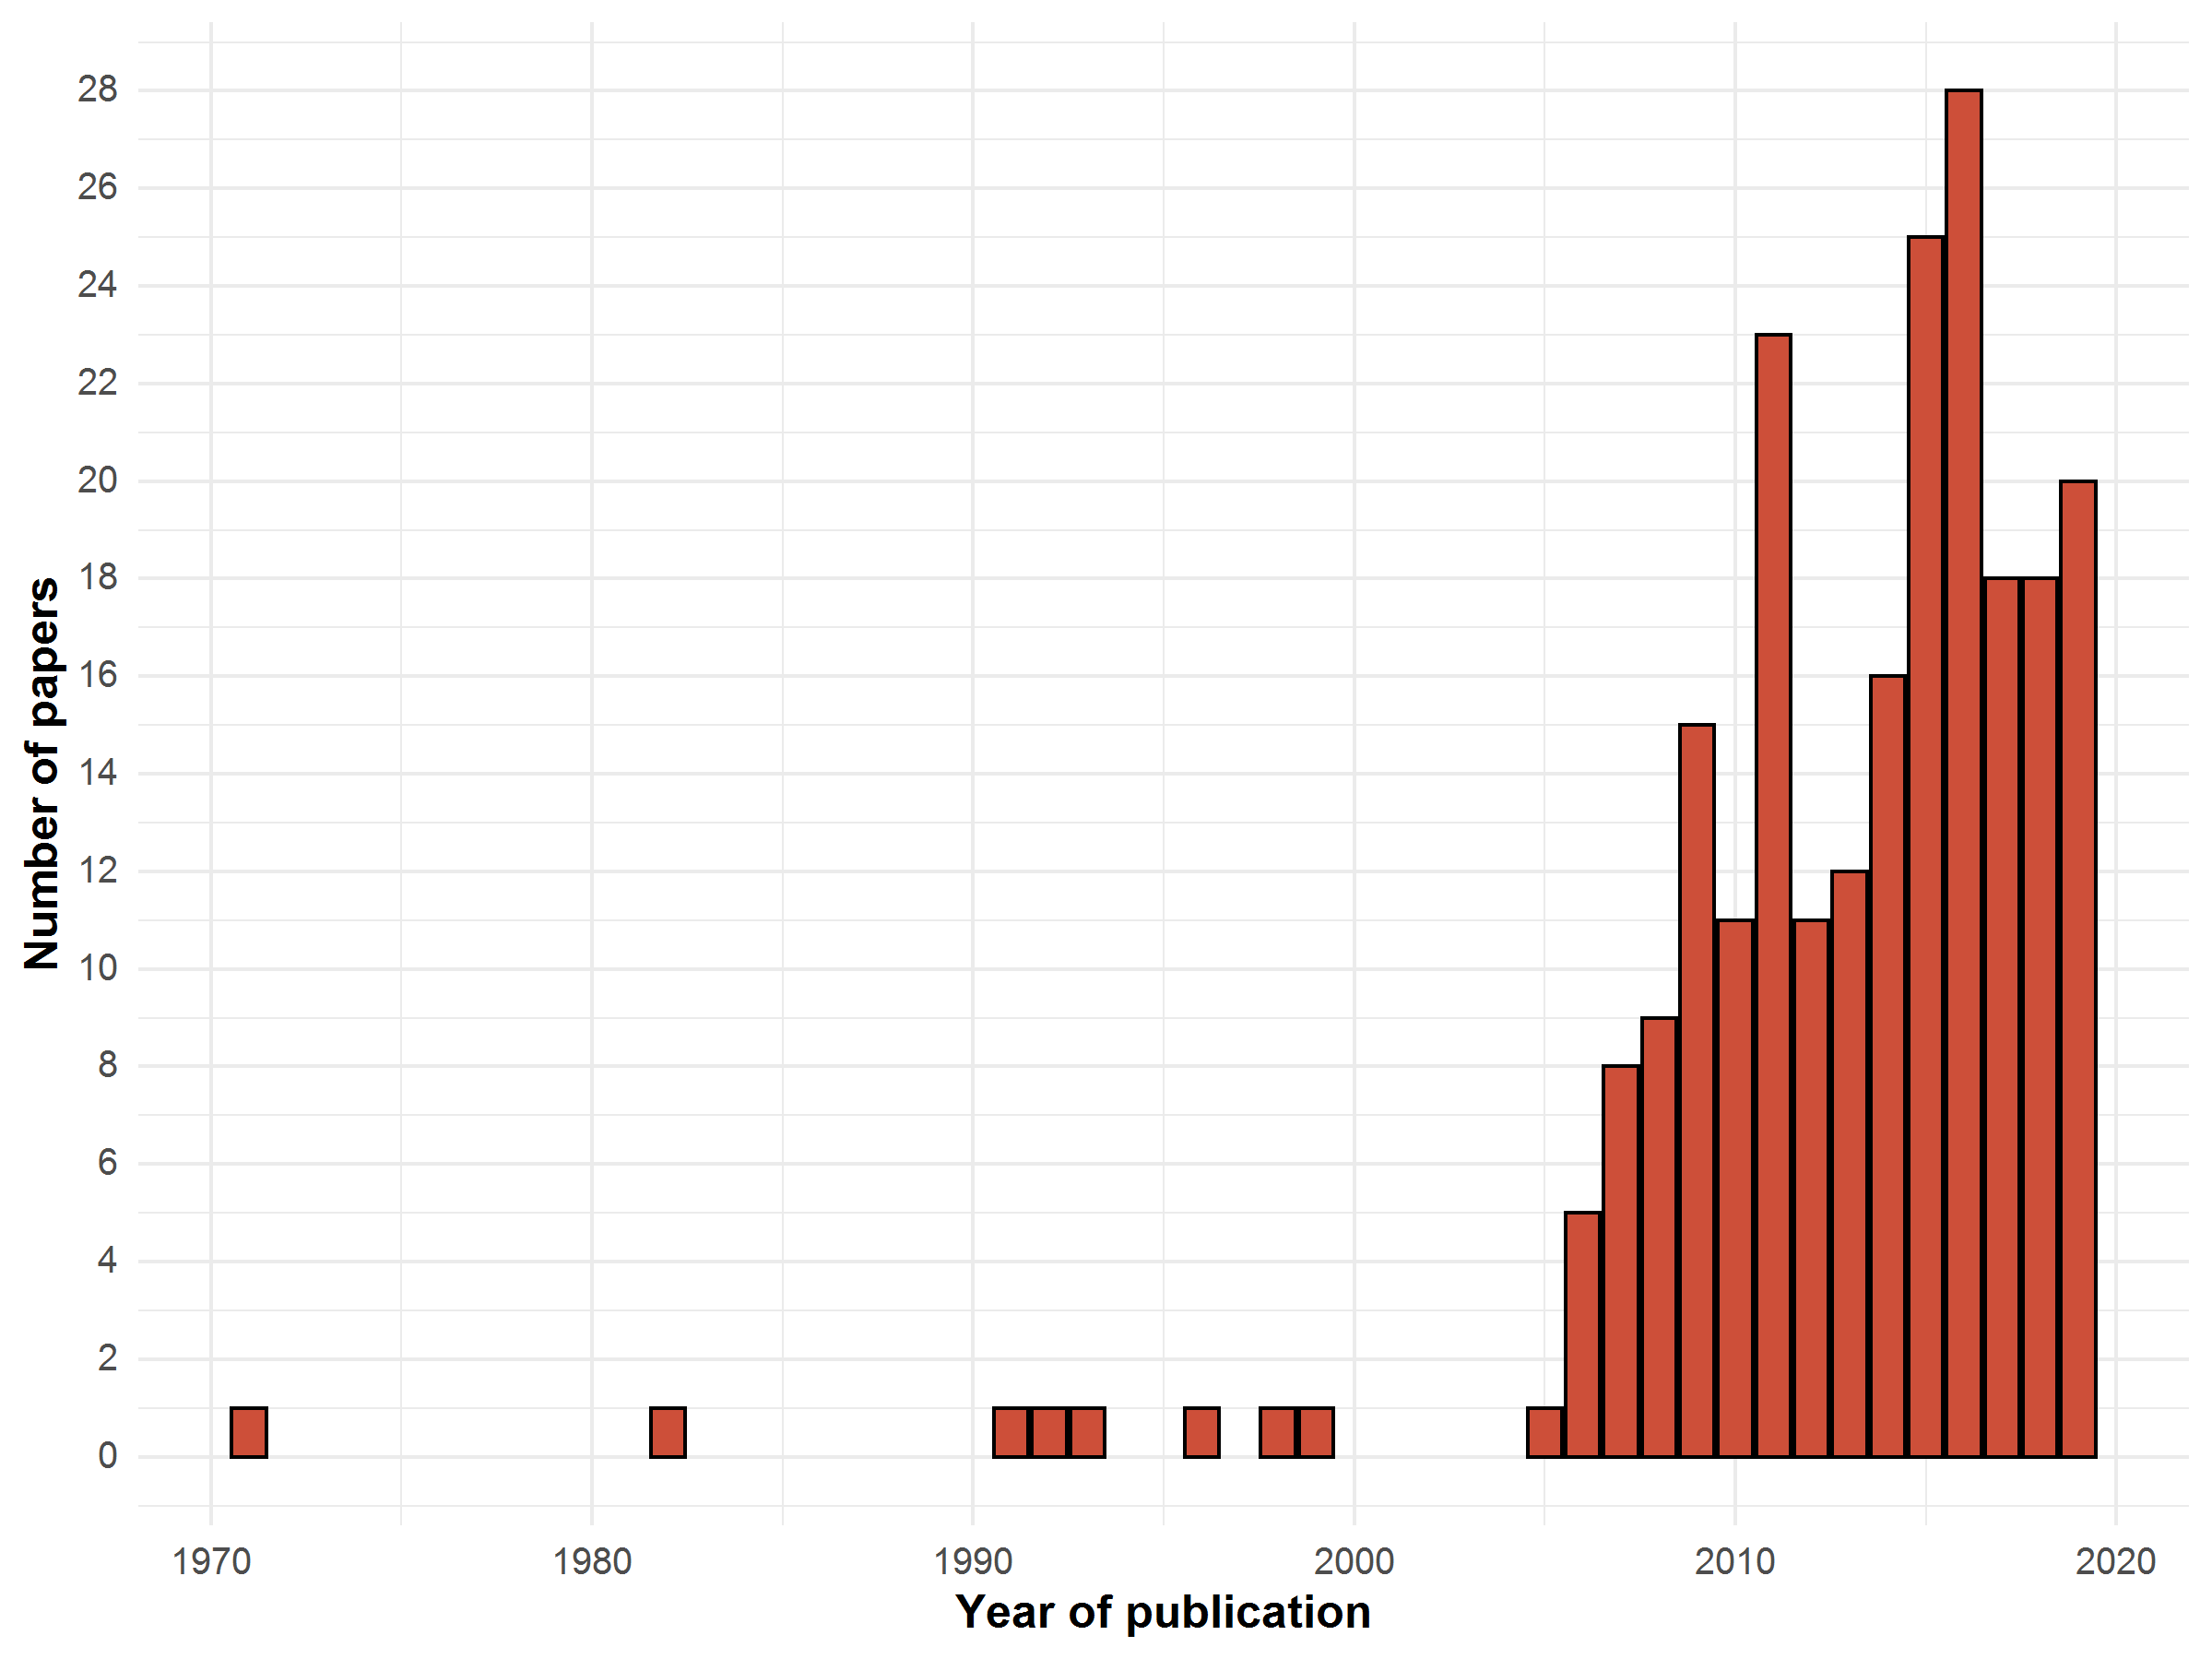
\includegraphics[scale=0.65]{figs/fig2_publications_per_year.png}
	\caption{\bf Number of publications per year (1970-2019).}
	\label{publications_per_year}
\end{figure}

We first categorised the papers according to the unique combinations of author affiliation types (Table \ref{studies_per_author_affiliations_type}). 

Overall, papers with only authors from academic institution affiliations were the most common (56.1\%; 128/228). Papers with author affiliations from academic and governmental organization affiliations were the second most common (25.0\%; 57/228), and followed by those with academic and NGO affiliations (7.5\%; 17/228). The least common were those with governmental and NGO affiliations (0.9\%; 2/228).

As explained earlier, we ultimately grouped the author affiliation combinations into two collaboration types. There were more purely academic collaborations (56.1\%; 128/228) than mixed collaborations (43.9\%; 100/228). 

\begin{table}[!h]
\centering
\caption{\bf Number of studies per unique combination of author affiliations (human diseases). Here, we also show the grouping of author affiliation combinations into purely academic and mixed collaborations. Purely academic collaborations refer to those authored by only authors with academic institution affiliations whereas mixed collaborations include those authored by a mixture of authors with academic institution affiliations, government institutions, and NGOs or only one of the last two.}
\setlength\arrayrulewidth{1pt} 
\begin{tabular}{|l l c|}
\hline
\textbf{Collaboration type} & \textbf{Author affiliation combination} & \textbf{Number of publications} \\ \hline
Purely academic & academic only  & 128 \\ \hline
Mixed & academic + governmental   & 57 \\ \hline
Mixed & academic + NGO                 & 17  \\ \hline
Mixed & academic + governmental + NGO    & 14 \\ \hline
Mixed & governmental only                & 5 \\ \hline
Mixed & NGO only                       & 5  \\ \hline
Mixed & governmental + NGO               & 2 \\ \hline  \rowcolor{gray!20}
\textbf{Total} &  & \textbf{228} \\  \hline 
\end{tabular}
\label{studies_per_author_affiliations_type}
\end{table}

To investigate the changes in collaboration types over time, we calculated the number and proportion of studies per collaboration type per year (Fig \ref{studies_per_collab_type}). In the past seven years (2013-2019), there was an absolute increase in the number of papers by both collaboration types. However, in the same period, there was no increase in the relative proportion of publications per year of mixed collaborations (\nameref{S1_Fig}).

\begin{figure}[!h]
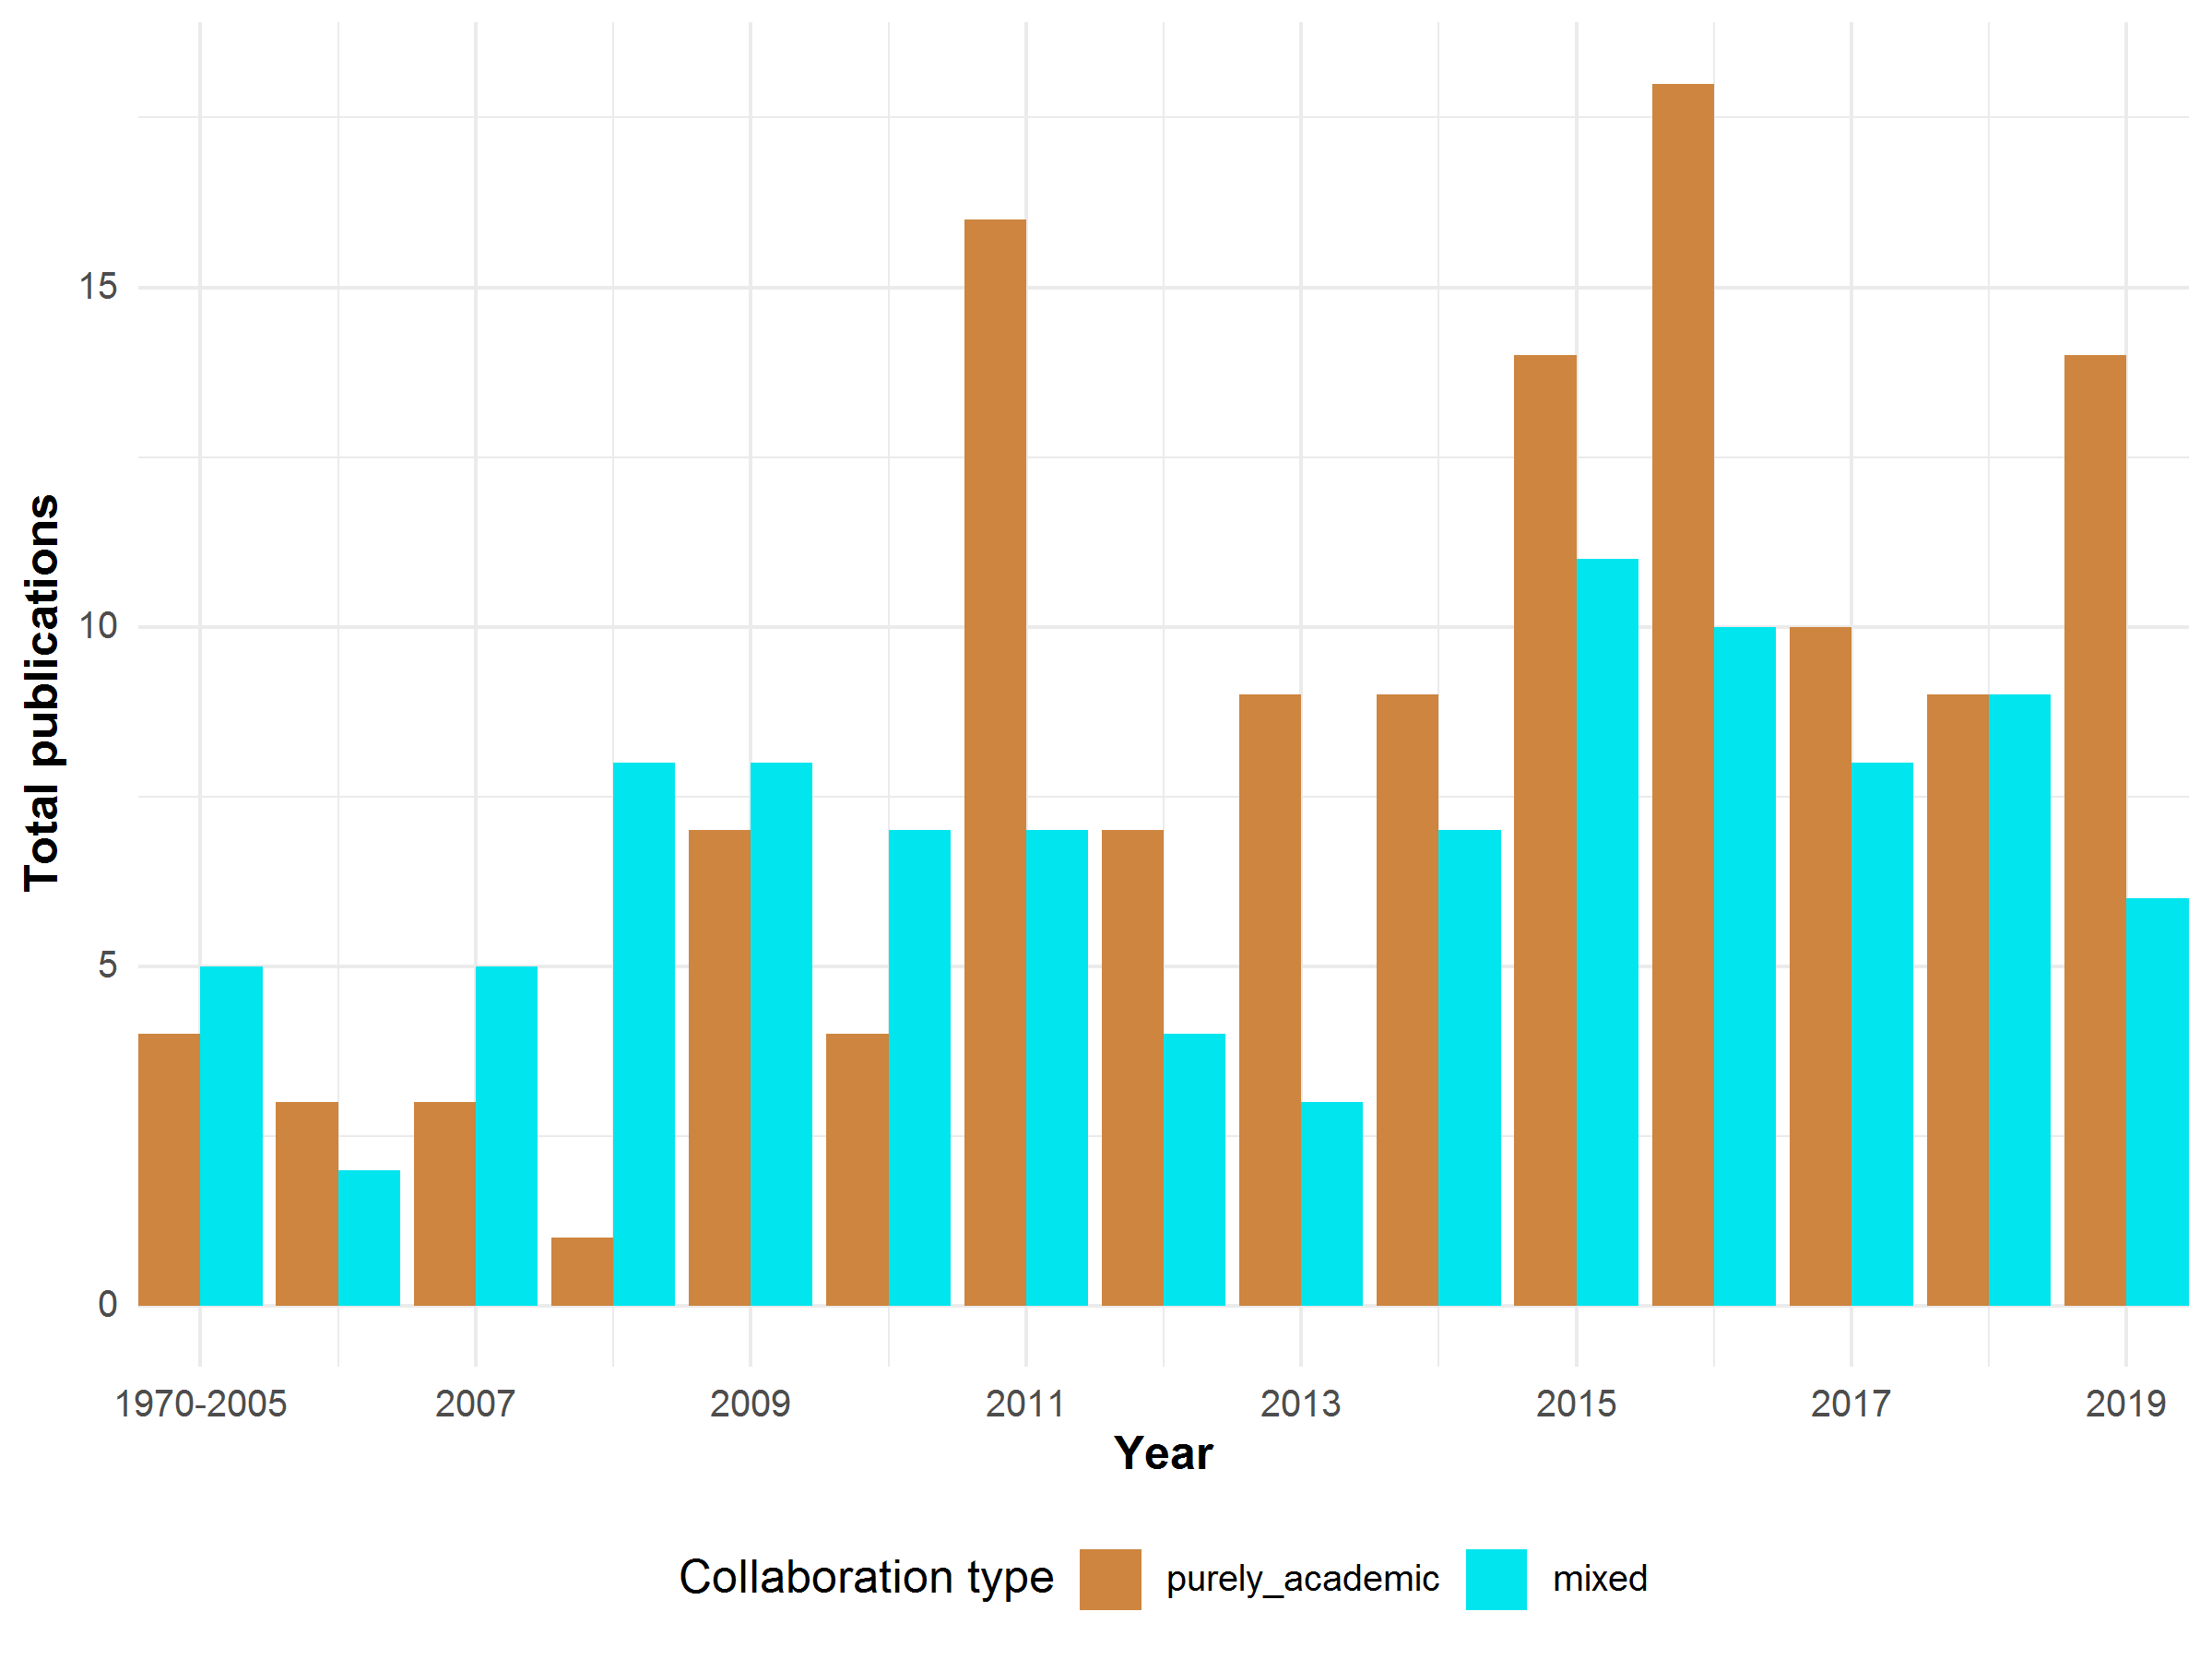
\includegraphics[scale=0.65]{figs/fig3_total_collabs_per_year_plot.png}
	\caption{\bf Total studies by collaboration type. The period from 1970-2005 has been lumped up due to the lack of publications. Academic collaborations refer to those authored by only authors with academic institution affiliations whereas mixed collaborations include those authored by a mixture of authors with academic institution affiliations, government institutions, and NGOs. Mixed collaborations are represented by the turquoise bars and purely academic collaborations by the brown bars.}
	\label{studies_per_collab_type}
\end{figure}

\subsection*{Locations studied}
Overall, most of the papers were about actual locations $(78.6\%; 195/248)$. Among these, some studied a geographic location spanning more than one country but not classifiable as a continent $(9.7\%; 19/195)$. Among those 19 studies, West Africa was studied the most $(47.4\%; 9/19)$, followed by the whole globe $(36.8\%; 7/19)$, Southeast Asia $(10.5\%; 2/19)$, and the Northern Hemisphere $(5.3\%; 1/19)$. 

When aggregated into continents, the Americas were studied the most $(36.4\%; 68/187)$, followed by Asia $(25.1\%;47/187)$, Africa $(24.6\%; 46/187)$, Europe $(13.4\%; 25/187)$, and Oceania $(0.5\%; 1/187)$.

When disaggregated into countries, the United States was the most studied $(21.1\%; 37/176)$, followed by China $(10.8\%; 19/176)$, Canada $(6.2\%; 11/176)$, and Sierra Leone $(5.7\%; 10/176)$.

\subsection*{Connection of authors to the location studied}
We investigated the connection of the authors to the location studied and found that, overall, there were more studies with at least one author connected to the studied location $(75.2\%; 118/157)$ than not $(24.8\%; 39/157)$. 

When stratified by collaboration types, mixed collaborations were more likely to have studies with at least one author in the location studied $(83.1\%; 63/77)$ compared with the purely academic collaborations $(67.5\%; 54/80)$. 

\subsection*{Diseases studied}
Overall, the number of studies per disease was disproportionately distributed (Table \ref{studies_per_disease_and_collaboration_type}). Influenza was the most studied $(57.2\%; 135/236)$, followed by Ebola $(14.4\%; 34/236)$, Dengue $(5.1\%; 12/236)$, and a tie between Cholera $(4.7\%; 11/236)$, and Measles $(4.7\%; 11/236)$. 

When the diseases were broken down in terms of collaboration type, there were clear differences in their distribution. Influenza, Dengue, and Measles were more studied by mixed collaborations whereas Ebola and Cholera were more studied by purely academic collaborations. 

\begin{table}[!h]
		\setlength\arrayrulewidth{1pt} 
	\centering
	\caption{\bf Number of studies per disease and collaboration type. Percentages are calculated from the row totals. The number of studies making up the percentages are shown in brackets. In counting the number of papers per disease studied, if a study was about more than one disease, we treated each instance as unique and counted them separately, leading to a total greater than the reported number of studies.}
	\label{chap3-table: Number of studies per disease and collaboration type}
	\begin{tabular}{|l c c c|}
		\hline
		\textbf{Disease}         & \textbf{Purely academic} & \textbf{Mixed} & \textbf{Total} \\ \hline
		Influenza                & 52.6\% (71)     & 47.4\% (64) & 135   \\ \hline
		Ebola                    & 70.6\% (24)     & 29.4\% (10) & 35    \\ \hline
		Dengue                   & 50.0\% (6)      & 50.0\% (6)  & 12    \\ \hline
		Cholera                  & 81.8\% (9)      & 18.2\% (2)  & 11    \\ \hline
		Measles                  & 36.4\% (4)      & 63.6\% (7)  & 11    \\ \hline
		Tuberculosis             & 85.7\% (6)      & 14.3\% (1)  & 7     \\ \hline
		Poliomyelitis            & 28.6\% (2)      & 71.4\% (5)  & 7     \\ \hline
		Varicella                & 50.0\% (2)      & 50.0\% (2)  & 4     \\ \hline
		Meningococcal meningitis & 33.3\% (1)      & 66.7\% (2)  & 3     \\ \hline
		Pertussis                & 50.0\% (1)      & 50.0\% (1)  & 2     \\ \hline
		Pneumococcal disease     & 50.0\% (1)      & 50.0\% (1)  & 2     \\ \hline
		Yellow fever             & 50.0\% (1)      & 50.0\% (1)  & 2     \\ \hline
		Hepatitis A             & 100.0\% (1)     & 0.0\% (0)   & 1     \\ \hline
		Rubella                  & 100.0\% (1)     & 0.0\% (0)   & 1     \\ \hline
		Typhoid                  & 100.0\% (1)     & 0.0\% (0)   & 1     \\ \hline
		Hepatitis B              & 0.0\% (0)       & 100.0\% (1) & 1     \\ \hline
		Malaria                  & 0.0\% (0)       & 100.0\% (1) & 1     \\ \hline
		Mumps                    & 0.0\% (0)       & 100.0\% (1) & 1    \\ \hline \rowcolor{gray!20}
		\textbf{Overall}			&	\textbf{55.5\% (131)}   			& \textbf{44.5\% (105)}   & \textbf{100\% (236)} \\
		\hline
	\end{tabular}
	\label{studies_per_disease_and_collaboration_type}
\end{table}

\subsection*{Intervention types and impact of vaccination}
There were more papers about non-vaccination interventions $(48.2\%; 110/228)$, followed by those that modelled vaccination as part of a mix of interventions or do-nothing counterfactuals $(41.7\%; 95/228)$, and those that modelled vaccination as a single intervention for side-by-side comparison with other non-vaccination interventions $(10.1\%; 23/228)$. 

The third group of papers that modelled vaccination as a single intervention allowed us to collate conclusions on the sole impact of vaccination. There were approximately the same number of studies in this set of studies belonging to the two collaborations types. 

Concerning the conclusions about the sole impact of vaccination as a single intervention, most of the studies found vaccination to be the most impactful single intervention in side-by-side comparison with other non-vaccination interventions $(82.6\%; 19/23)$. Few studies found the vaccination to be less impactful compared to other interventions and for various reasons $(17.4\%; 4/23)$. Influenza was the disease studied in these latter four cases. Isolation, and antivirals were found to be more impactful than vaccination due to reasons including the delay until a strain-specific vaccine is developed to control the disease. 

\subsection*{Model structure, spatial heterogeneity, and model dynamics}
There were more compartmental models $(78.5\%; 179/228)$ than agent-based models $(20.2\%; 46/228)$ with no clear difference in preference between the two collaboration types. 

Approximately a third of the papers included spatial heterogeneity $(28.9\%; 66/228)$ with no clear difference between the two collaboration types. 

Deterministic models were the most common $(62.3\%; 142/228)$ compared to stochastic $(31.6\%; 72/228)$ and hybrid models $(6.1\%; 14/228)$, that is models with both deterministic and stochastic components. Here, mixed collaborations were more likely to use stochastic models $(40.0\%; 40/100)$ than purely academic collaborations $(25.0\%; 32/128)$. 

\subsection*{Model parametrization and validation}
The top three most commonly used parametrization methods included: combining literature sources and expert opinion/assumptions, literature sources and fitting to data, and literature sources only (Table \ref{model_parametrization_results}). 

The most common parametrization method among mixed collaborations was the combination of literature sources and fitting $(27.3 \%; 35/128)$, whereas the combination of literature and expert opinion was the most common among purely academic collaborations $(28.0\%; 28/100)$. 

\begin{table}[!h]
\setlength\arrayrulewidth{1pt} 
\centering
\caption{\bf Model parametrization methods. We define parametrization as the method of determining the parameter values for the model. In the table, ``Literature'' means the model's parameters were obtained from literature sources. ``Expert opinion'' means the values were assumed in consultation with experts of the field. ``Fitted'' means the model’s parameters were obtained through some form of mathematical or statistical fitting to a time series of data. }
\begin{adjustwidth}{-2.10in}{0in}
\begin{tabular}{| p{0.17\textwidth}  p{0.14\textwidth}  p{0.14\textwidth}  p{0.12\textwidth}  p{0.13\textwidth}  p{0.13\textwidth}  p{0.12\textwidth}  p{0.1\textwidth}  p{0.07\textwidth} |} \hline 
\textbf{Collaboration type} & \textbf{Literature and expert opinion} & \textbf{Literature and fitted} & \textbf{Literature} & \textbf{Expert opinion} & \textbf{Literature, expert opinion, and fitted} & \textbf{Fitted} & \textbf{Expert opinion and fitted} & \textbf{Total} \\ \hline
Academic & 27.3\% (35) & 22.7\% (29) & 18.0\% (23) & 13.3\% (17) & 9.4\% (12)  & 7.0\% (9) & 2.3\% (3) & 128 \\ \hline
Mixed & 25.0\% (25) & 28.0\% (28) & 15.0\% (15) & 7.0\% (7) & 19.0\% (19) & 5.0\% (5) & 1.0\% (1) & 100 \\ \hline \rowcolor{gray!20}
Overall & 26.3\% (60) & 25.0\% (57) & 16.7\% (38) & 10.5\% (24) & 13.6\% (31) & 6.1\% (14) & 1.8\% (4) & 228 \\ \hline 
\end{tabular}
\end{adjustwidth}
\label{model_parametrization_results}
\end{table}

Most studies did not perform any form of validation $(63.2\%; 144/228)$. Approximately a third used data to validate their models $(34.6\%; 79/228)$ (Table \ref{model_validation_results}). Mixed collaborations were more likely to validate their model with data or the output of an independent model. 

\begin{table}[!h]
	\centering
	\setlength\arrayrulewidth{1pt} 
	\caption{\bf Model validation methods. We define model validation as the method by which the model's performance was measured. ``None'' means no validation was performed, or the model’s output was compared to another output from the same model. ``Data'' means the model was compared to independently observed data. ``Another model’s output'' means the model's output was compared to an independent model's output.}
	\begin{adjustwidth}{-0.00in}{0in}
		\begin{tabular}{| p{0.15\textwidth}  p{0.13\textwidth} p{0.13\textwidth} p{0.13\textwidth} p{0.13\textwidth} p{0.12\textwidth}|}
			\hline
			\textbf{Collaboration type} & \textbf{None} & \textbf{Data} & \textbf{Another model's output} & \textbf{Data and another model} & \textbf{Total} \\ \hline
			Academic & 70.3\% (90) & 28.9\% (37) & 0.8\% (1) & 0.0\% (0) & 128 \\ \hline
			Mixed & 54.0\% (54) & 42.0\% (42) & 3.0\% (3) & 1.0\% (1) & 100 \\ \hline \rowcolor{gray!20}
			Overall & 63.2\% (144) & 34.6\% (79) & 1.8\% (4) & 0.4\% (1) & 228\\ \hline
		\end{tabular}
	\end{adjustwidth}
	\label{model_validation_results}
\end{table}


\subsection*{Data and model simulation code}
More than half of the papers used datasets collected independent of the study for either the model parametrization or validation process $(56.1\%; 128/228)$. These papers were split approximately equally between the two collaboration types. 

The use of accessible data was, however, different between the two groups. Purely academic collaborations were more likely to use data that could be accessed in the public domain $(81.0\%; 51/63)$ compared to mixed collaborations $(56.9\%; 37/65)$.  

Few papers provided access to the model simulation code $(1.7\%; 4/228)$. Here, if a paper indicated that the authors could be contacted for the code, it was deemed as inaccessible due to the many hurdles with getting the code in time. Some papers reported the computer application/software/program/package used (R, Python, C++, Matlab, and so forth) but we did not collect that information. 

\subsection*{Patterns in the foot and mouth disease (FMD) literature}
There were $25$ studies about foot and mouth disease outbreaks. Due to the small number of studies, the absolute differences between the two collaboration types were generally not large enough to be considered (\nameref{S2_File}), hence, we report on the aggregated patterns. 

In terms of collaboration types, slightly more than half of the $25$ studies were authored by mixed collaborations $(56.0\%; 14/25)$ than purely academic collaborations $(44.0\%; 11/25)$. Almost all the papers had at least one author in the location studied $(92.0\%; 23/25)$. 

Overall, vaccination was modelled as a single intervention for comparison in more than half of the studies $(56.0\%; 14/25)$, followed by vaccination in combination with other interventions $(28.0\%; 7/25)$, and no vaccination $(16.0\%; 4/25)$. Few of the first set of studies found vaccination to be the most impactful as a single intervention $(14.3\%; 2/14)$.  

In general, the FMD models had more agent-based $(76.0\%; 19/25)$ and spatially explicit structure $(72.0\%; 18/25)$, largely used stochastic dynamics $(56.0\%; 14/25)$, and performed more sensitivity analyses $(56.0\%; 14/25)$. 

In terms of model parametrization, the most common method was the combined use of literature sources and expert opinion $(28.0\%; 7/25)$, followed by fitting to data only $(20.0\%; 5/25)$, and the combined use of literature sources, expert opinion, and fitting to data $(16.0\%; 4/25)$. Here, mixed collaborations were more likely than purely academic collaborations to combine literature sources and expert opinion $(42.9\% 6/14)$. Furthermore, most of the FMD models were not validated $(72.0\%; 18/25)$.


\section*{Discussion}
For the period $1970-2019$, co-authorship by purely academic collaborations formed over $56\%$ of the outbreak response impact modelling studies of human vaccine-preventable diseases. Both collaboration types increased in absolute numbers over the past seven years. Regarding modelling practices between the two collaboration types, mixed collaborations were more likely to: (i) include authors affiliated through their institutions to the location studied, (ii) use more complex modelling practices including stochastic model dynamics, parametrization methods involving a combination of literature sources, expert opinion/assumptions, and fitting to data, and validate their models with data collected independent of the study. Even though this review was about human vaccine-preventable diseases, only 51.8\% of the studies modelled vaccination in some form. Moreover, only 10.1\% of the total studies modelled vaccination for comparison with other non-vaccination strategies in the same analysis. Influenza was disproportionately the most studied disease, followed by Ebola, and Dengue. 

There were several differences in models and practices between the human disease literature and foot and mouth disease (FMD). Mixed collaborations dominated the FMD literature, with almost all papers having an author in the location studied. Furthermore, most of the FMD models and modelling practices were more complex involving the use of spatial, stochastic, agent-based models. However, the FMD models were less likely to be validated with real world data.

Collaborations, especially between authors from academic institutions, governmental, and non-governmental organizations responsible for outbreak response, could lead to knowledge transfer and improved decision-making \cite{Muscatello2017}. Moreover, such diversity in modelling collaborations could expand the skill sets needed to solve the complex real world outbreak response needs. However, it is well known that there is a weak link between academic research and decision-making in general, and research findings are often not easily translated into decisions \cite{Choi2005,Deelstra2003,Muscatello2017}. This gap in knowledge translation exists especially between outbreak response researchers and public health decision-makers \cite{Rivers2019,Muscatello2017}. There are examples of the commissioning of modelling by organisations such as the US Centers for Disease Control and Prevention (CDC) and the World Health Organization (WHO) to inform decision-making during past outbreaks of Influenza, Ebola, Zika, and Dengue \cite{Muscatello2017}. However, many decision-makers remain cautious about the uptake of modelling due, in part, to issues about transparency in assumptions, credibility and ease of use of modelling software, and adaptability of the results to other settings and existing policies \cite{Muscatello2017}.

To bridge this knowledge translation gap between modellers and decision-makers, modelling collaborations that deepen the interaction between model developers and decision-making have been proposed \cite{Choi2005,Rivers2019}. This could be achieved through the sharing of expertise so that the academics formulate, parametrize, and validate the models taking into account the expert opinions of the decision-makers so that the findings are more tailored towards implementation. Mixed or interdisciplinary collaborations have been reported to be strongly associated with research impact and translation to decision-making \cite{Deelstra2003}. Hence, outbreak response, which is broadly an operational field, would ideally have modelling groups/collaborations that are comprised of academics and decision-makers to bridge this gap. In this review, we observed an absolute increase in the number of papers published by mixed collaborations (Fig \ref{studies_per_collab_type}). This could suggest an increase in the uptake or recognition of modelling as an outbreak response decision-making tool. Future research to investigate and explain this increase could advance our understanding of the contribution of modelling to outbreak response decision-making.

The inclusion of local experts in outbreak response modelling teams helps with more tailored problem-solving and decision-making and better reception of the decisions made \cite{Abramowitz2015}. In that regard, mathematical modelling collaborations involving local experts or, in this review, locally affiliated co-authors are an important first step towards achieving this. We found that most of the human disease studies had authors with an institutional affiliation in the location studied. We observed the same pattern for FMD albeit at a much higher percentage. However, when the human disease data were disaggregated, the results showed that mixed collaborations had a much higher percentage of studies with at least one author in the studied location compared to purely academic collaborations. Coupling this with the absolute increase in publications by mixed collaborations in the past seven years could suggest an increase in the uptake of modelling as a public health decision-making tool. However, we did not measure this causality. Research that measures the direct impact of mathematical modelling in public health decision-making remains lacking in the literature \cite{Muscatello2017}. Future studies designed to investigate this uptake of models and whether it has had an impact on outbreak response would contribute meaningfully to the field of outbreak response modelling. 

Three classes of interventions with respect to vaccination were modelled: non-vaccination (mostly antiviral use and non-pharmaceutical interventions), vaccination mixed with other complementary non-vaccination interventions, and vaccination as a single intervention for side-by-side comparison with other non-vaccination alternatives. The last class of interventions were the only eligible set for our analysis of the conclusions about whether vaccination is always the most impactful intervention when modelling is used as the assessment tool. Even though all the reviewed studies were about human vaccine-preventable diseases, only 10.1\% of the studies modelled vaccination as a single intervention for side-by-side comparison with non-vaccination interventions. This lack of studies assessing the sole impact of vaccination reflects the reality that vaccination is often  implemented alongside other interventions and never alone, making it difficult to assess its sole impact. Nevertheless, mathematical modelling is an ethically viable way to assess the sole impact of vaccination, and hence, an essential tool for decision-making.  

Among the studies that modelled vaccination as a single intervention for comparison with other single non-vaccination interventions, vaccination was found to be the most impactful intervention in 82\% of the studies. Four studies out of the 23 that modelled influenza found case isolation \cite{Yasuda2009,Gao2016,Chen2020a} and antiviral prophylaxis and/or therapeutics \cite{Gumel2008} to be more impactful than vaccination assuming those interventions could be implemented immediately, given significantly efficient isolation and large antiviral stockpiles before the outbreak/pandemic. Among these four studies, some common assumptions that influenced how vaccination was implemented included: the late arrival of effective vaccines \cite{Yasuda2009}, low versus high vaccination rates \cite{Gao2016}, the use of partially effective pre-existing vaccines against the current strain reactively \cite{Gumel2009} or pre-emptively \cite{Chen2018}. In all four studies, it was, however, recommended that, vaccination be used in combination with the alternative interventions. Even though antivirals were found to be more impactful in some cases, its prolonged use was discouraged to prevent the development of antiviral resistance \cite{Gumel2009}. On the other hand, there was a high percentage of studies in the FMD literature about the use of vaccination as a single intervention and vaccination was rarely found to be the most impactful intervention. 

We found some commonalities and differences in the choice of model structure and dynamics between the two collaboration types in the human disease literature. Mixed collaborations were more likely to use ``complex'' models and practices. We are not making any value judgements with regards to complexity but are only highlighting these differences that might require further investigation. Moreover, it is common to model an outbreak using alternative model choices and assumptions depending on the question being answered \cite{Basu2013}. However, the results must always be interpreted with cognisance of the limitations/assumptions of the model.  The use of more complex models and practices by mixed collaborations is likely due to the fact that often, real world public health policy-related decision-making is operational, requiring finer details in models and approaches to answer the questions posed in a practical way. Our definition of mixed collaborations meant that it may have involved decision-makers. It is, therefore, likely that their need for practical solutions could have influenced higher levels of model details or complexity. 

The FMD models were generally more complex than the human disease models. This is not surprising because the nature of FMD spread often requires the inclusion of farm structure, farm connectivity, and demographics to capture the disease's dynamics accurately \cite{Kinsley2018}. Future studies designed to explain the differences in modelling practices of human outbreak response modelling groups might help to explain what we have observed in this review.

A little over half of the human disease papers used observed data for parametrization or validation. Additionally, only 4 studies shared their code in an easy to access form. On the other hand, the FMD models were generally not validated with observed data. Owing to this, it might be difficult to reproduce some of the results in these outbreak response modelling studies. We recognise that data sharing in public health raises a lot of debate regarding privacy and intellectual property, and often, authors are hindered by institutional data sharing policies \cite{Kim2016}. We, however, recommend that data and code be shared where possible to promote open science practices that help advance the field.  

This review had several limitations. First, outbreak response models and analyses are not always published in peer-reviewed journals, but this systematic review only focussed on peer-reviewed articles. It is, therefore, possible that some relevant studies were missed by our search strategy. Second, we used the author list and affiliations to classify studies as either purely academic or mixed. However, this could cause some mixed collaborations to be misclassified as purely academic, especially in cases where non-academics contributed to papers classified as purely academic but were not included on the author list. It is, however, standard practice to include individuals who contributed substantially to a piece of scientific writing, hence, if that was not done for a paper, it could imply that the level of interaction was not high enough to warrant the credit of authorship. Third, in the absence of an explicit measure of contribution of mathematical modelling to outbreak response decision-making, we used mixed collaborations as a proxy. Thus, we may be under-estimating the number of mixed collaborations in the literature. Forth, we only surveyed the literature on a specific study design – mechanistic models. We excluded statistical models and other computational models, which are not mechanistic. Hence, the results of this systematic review should only be interpreted in the context of the mechanistic modelling landscape. Furthermore, it is also possible that some purely academic collaborations contribute to decision-making whereas some mixed collaborations are purely an academic exercise. Also, we  conducted our database searches in January 2020 and therefore do not reflect the literature, or any changes in practice, associated with the COVID-19 pandemic. Lastly, by only including papers published in English, we most certainly missed papers published in other languages.  

Numerous factors could explain the patterns we have observed in this review, and we would recommend future studies that will use appropriate study designs, for example, interviews of modelling groups and public health decision-makers, to explain why certain model choices and modelling practices were made by the collaboration types. Future studies should investigate when modelling results directly impacted decision-making and what determined that to identify best practices that will strengthen the link between modelling and decision-making in the future. We expect that collaboration between academia, decision-makers, and local experts will enhance decision-making by accounting for aspects of policy and decision-making that might be overlooked in studies conducted mainly as a theoretical exercise. 

\subsection*{Other information}
A protocol following the PRISMA guidelines for systematic review protocols and outlining the procedures for this systematic review was registered on PROSPERO with registration number CRD42020160803 and published through a peer-reviewed process~\cite{Azam2020}. 
 
\section*{Supporting information}

\paragraph*{S1 File}
\label{S1_File}
{\bf Search strings and results, data items extracted, and questionnaire for data extraction.} 

\paragraph*{S1 Fig}
\label{S1_Fig}
{\bf Collaboration patterns in time (proportions per year).}

\paragraph*{S2 File}
\label{S2_File}
{\bf Analysis of extracted data.} 

\paragraph*{S3 Table}
\label{S3_Table}
{\bf PRISMA checklist.} 

%\section*{Acknowledgments}

% Use the PLoS provided BiBTeX style
\bibliography{references.bib}
\bibliographystyle{vancouver}
\nolinenumbers
\end{document}

